

\typeout{Towards Artificial Intelligence for Metaphysics: \\ the Case of the Inconsistency in G\"odel's Ontological Argument}


\documentclass{article}
\usepackage{ijcai15}

% Use the postscript times font!
\usepackage{times}

% the following package is optional:
\usepackage{latexsym} 

\usepackage{amsmath}
\usepackage{modallogics}
\usepackage{graphicx,url}

\newcommand{\imp}{\rightarrow}
\newcommand{\biimp}{\leftrightarrow}
\newcommand{\allq}{\forall}
\newcommand{\exq}{\exists}
\newcommand{\seq}{\vdash}
\newcommand{\nec}{\Box} % necessarily
\newcommand{\pos}{\Diamond} % possibly

\title{Towards Artificial Intelligence for Metaphysics: \\ the Case of the Inconsistency in G\"odel's Ontological Argument}
\author{Christoph Benzm\"uller\thanks{German Research Foundation DFG \ldots} and Bruno Woltzenlogel Paleo}
\author{}

\begin{document}

\maketitle

\begin{abstract}
  This paper discusses the discovery of the inconsistency in G\"odel's ontological argument as a success story for artificial intelligence. Despite the popularity of the argument since the appearance of G\"odel's manuscript in 1970, the inconsistency of the axioms used in the argument remained unnoticed until 2013, when it was detected automatically by the higher-order theorem prover LEO-II. Understanding and verifying the refutation generated by the prover turned out to be a time-consuming task, and its completion, as reported here, required the reconstruction of the refutation in the Isabelle proof assistant. The development of an improved syntactical hiding for the embedding technique, utilizing Isabelle's binding notation mechanism, allows the refutation to be presented in a human-friendly way, suitable for non-experts in the technicalities of the higher-order theorem proving. This brings us a step closer to wider adoption of logic-based artificial intelligence tools by philosophers.
\end{abstract}


\section{Introduction}
Without exaggeration Kurt G\"{o}del's ontological
argument for the existence of God \cite{GoedelNotes,ScottNotes} is
amongst the most discussed formal proofs in modern literature. A rich
body of publications -- including very recent ones -- present,
discuss, assess, criticise, modify and improve G\"{o}del's original
work (see e.g.~Sobel~\shortcite{Sobel} and Oppy~\shortcite{sep-ontological-arguments} and the
references therein).  In philosophy lectures at universities the
argument is regularly presented as a masterpiece argument in
metaphysics. Since 2013, when Benzm\"uller and Woltzenlogel-Paleo~\shortcite{J30,C40} first
reported their successful initial computer-assisted
analysis of G\"odel's proof and Scott's variant,
their work has received a media repercussion on a global scale\footnote{A
  small collection of news articles is available at {\scriptsize
    \url{https://github.com/FormalTheology/GoedelGod/blob/master/Press/LinksToNews.md}}},
and numerous bloggers commented on the proof
\cite{fuhrmann15:_blogg_goedel}.

The in-depth computational analysis presented here substantially
extends previous computer-assisted studies of G\"odel's ontological
argument. Similar to the related work \cite{J30,C40} the analysis has
been conducted with automated theorem provers for classical
higher-order logic (HOL) even though G\"odel's proof is actually
formulated in \emph{modal} higher-order logic. To bridge between the two
logics we utilise and further improve the logic embedding
approach \cite{J23,C40}, which has already been employed succesfully in preceding related work.


The novel contributions reported in this paper include the following:


\begin{itemize}
\item A detailed analysis of the inconsistency of G\"{o}del's
  \shortcite{GoedelNotes} original version of the proof is presented
  for higher-order modal logics KB and K (with possibilist and
  actualist first-order quantifiers). The extraction, reconstruction
  and verification of an informal, human intuitive argument has been
  an open problem since the first detection of this inconsistency by
  Benzmüller and Woltzenlogel-Paleo \shortcite{C40} with the LEO-II prover. 
  The experiments reported here led to the discovery of a surprisingly accessible
  understanding of this inconsistency which is philosophically
  profound and which has not been presented yet in the
  literature. The detection of this inconsistency in combination with
  the work reported here thus demonstrates that artificial intelligence systems -- 
  particularly higher-order automated
  theorem provers -- are capable of assisting in the discovery and ellucidation of
  \emph{new} and philosophically relevant knowledge. 
\item Another open question has been whether the final theorem T3 \textit{``Necessarily, there
    exists God''} could eventually be proved fully automatically
  directly from the axioms alone. In \shortcite{C40}, the provers had only succeeded in proving 
  T3 from intermediate argumentation steps (lemmata). Here we report that, by using a more efficient new
  embedding for the higher-order modal logic S5, T3 can be directly proven from Scott's version of the axioms, which are consistent. The fully automatic proof has been
  generated by the theorem prover \textsc{Leo-II}~\cite{C26} and
  subsequently verified in the proof assistant
  Isabelle/HOL~\cite{NPW02}.
\item A third open challenge the verification in Isabelle/HOL of the modal
  collapse \cite{Sobel}, which is one of the most strongly criticised
  `side-effects' of G\"odel's and Scott's variants of the proof. In previous work
  the modal collapse has been derived by the provers
  \textsc{Satallax} \cite{Satallax} and \textsc{Leo-II}, but a fully automatic
  verification in the highly trusted Isabelle/HOL still failed. 
  Now, with the more efficient embedding for S5, this verification has been done. 
\item On the technical side, we present a significantly improved
  syntax representation of G\"odel's resp.~Scott's proof in
  Isabelle/HOL. In fact, we demonstrate that a nearly perfect match
  between the original pen and paper presentations and our encoding in
  Isabelle/HOl is feasible. This is clearly an important prerequisite
  for promoting the theorem proving technology employed here to a wide community of
  philosophers, who are not necessarily experts in automated reasoning or higher-order logic.
\item On the other hand, we
  also point to several technical challenges which, at least for the
  moment, still restrain non-expert users of these systems from
  independently conducting similar experiments in computational
  metaphysics as reported here and in previous work. 
% Technical issues detected within Isabelle-Sledgehammer; room for improvements
\end{itemize}

% These novel contributions are presented in Sections ? and ?.
% In Section ?, novel and previous findings are summarised and discussed 
% with regard to their relevance in metaphysics. In this section also 
% some further details and improvements on earlier 
% findings are presented.
% Section ? concludes the paper.

Give paper structure (maybe not needed) ...


First successful applications of theorem proving technology in
metaphysics were reported by Oppenheimer and
Zalta~\shortcite{oppenheimera11}, who coined the term \textit{Computational Metaphysics} for this new research area and employed the first-order
\textsc{Prover9} \cite{Prover9} in their experiments. Later on, Rushby~\shortcite{rushby13} used the proof assistant \textsc{PVS} \cite{PVS}. Common to both
works is a significant amount of proof-hand-coding work as well as their
focus on a non-modal formalization of St. Anselm's~\shortcite{Anselm} simpler 
and older ontological argument. 
None of these previous works formalises and automates variants of \emph{higher-order} and \emph{modal} logics, which are, however, crucial
for G\"{o}del's more complex ontological argument.
x

\section{Variants of the Ontological Argument}
Short history, Anselm, Leibniz, etc.
\subsection{G\"{o}del's Proof Script}
\subsection{Scott's Variant}
\subsection{Recent Variants}
Dozens of contributions were published in the last four decades which
present variants of G\"odel's/Scott's proofs. In many cases the
motivation has been to remedy the modal collapse. Other authors are
simply interested in a critical assessment. Particularly interesting
from the perspective of this paper is that many literature
contributions unfortunately work with or refer to G''odel's original
definition of essence
$$ todo $$
This original version avoids the conjunct added by Scott expressing
that essential properties of an individual should be possessed by the
individual. As we show in this paper using this notion of essence
leads to an inconsistent axiom system, which in a classical setting of
course deserves no further attention, since from an inconsistent
system everything can be concluded, including God's existence and
non-existence simultaneously. In other words, these literature
contributions discuss variants of the argument which from a classical
logical perspective do not deserve any further attention.

We give here a list of examples:
\begin{itemize}
\item Anderson and Getting's 1996, p. 168 \cite[p.168]{AndersonGettings1968}
  use essence without conjunct.
\item  Hazen 1998, p.365 \cite[p.365]{Hazen1998} states: ``G\"odel left this
  clause out in [11], but this appears to have been an oversight--it
  is included in related manuscripts''. There is not mentioning of an
  inconsistency though.
\item Look???, p. 514
% \item Oppy 1996, p.226-227 \cite[p.226/227]{Oppy1996}, Oppy 2000, p. 364
%   \cite[p.364]{Oppy200}, Oppy 2008, p. 1068 \cite[p.1068]{Oppy2008}:
%   Oppy uses: ``A is an essence of x iff for every property B, x has B
%   neces- sarily iff A entails B'' (this is from Anderson's
%   emendation). Check is this leads to inconsistency as well. In this
%   case we may write something like: 

%  Oppy presents an critical
%   assessment in order to conclude that G\"odel's argument fails to
%   convince. Oppy apparently does not see that he is assessing an
%   inconsistent axiom system (and he in fact creates adaptations that
%   suffer the same problems).
% \item 
\end{itemize}


\footnote{Fuhrmann2005: Gödel vermerkt diese Konsequenz [dass aus der Definition unmittelbar folgt, daß alle wesentlichen
Eigenschaften notwendig äquivalent sind] in einer Fußnote zur Definition. Die Definition selbst aber läßt im Definiens das Konjunkt Xx aus. Ohne das Konjunkt folgt jedoch die Konsequenz nicht. Es ist deshalb naheliegend anzunehmen, daß Gödel die Definition so beabsichtigte, wie sie hier notiert ist und wie Gödel sie selbst in früheren Notizbucheintragungen formuliert hat.}





\section{Automating HOML in HOL}
\subsection{Outline of the Embedding}
Logic textbooks commonly utilise classical higher-order logic (HOL)
\cite{Church} as a meta-language to introduce the syntax and the
semantics of object logics of interest, in which then reasoning
problems in concrete application domains can be modeled and solved
with pen and paper.  In fact, this approach can also be followed to
enable interactive and automated proof for even very challenging
objects logics with existing theorem provers for classical
higher-order logic.

% Just as commonly the case in logic textbooks, in the embeddings
% approach classical higher-order logic is utilised as a meta-language
% to encode the syntax and the semantics of object logics in which the
% proof problems of interest are then modeled in. Modulo the embedding
% state of the art automated theorem provers for classical higher-order
% logic can then be utilised as object logic reasoning tools.

For a computational analysis of G\"odel's ontological argument in this
approach the embedding of modal higher-order logics (MHOL) such as K,
KB and S5 for different domain conditions (possibilist and actualist)
is required. This idea has been successfully followed in related work
\cite{C40}. The embedding of modal higher-order logic is in fact
straightforward. Formulas in MHOL such as are lifted to predicates
over worlds, which are explicitly represented in the approach as
terms. Propositional MHOL such as $\neg \varphi$, $\varphi\vee\psi$
and $\box \varphi$ are then mapped to HOL formulas \ldots.  

It is easy
to see that this captures the standard translation \cite{Ohlbach},
which is here (intra-logically) realised in HOL by stating a set of
equations; see also Fig. ~\ref{QMLS5}. New is that also quantifiers 
can be mapped \ldots 

The approach is very flexible, KB, S5, domain conditions\ldots 


\subsection{Improved Embedding for S5}
We present an improved embedding (syntax and defintion of box) in  Fig.~\ref{QMLS5}).
\begin{figure}
\centerline{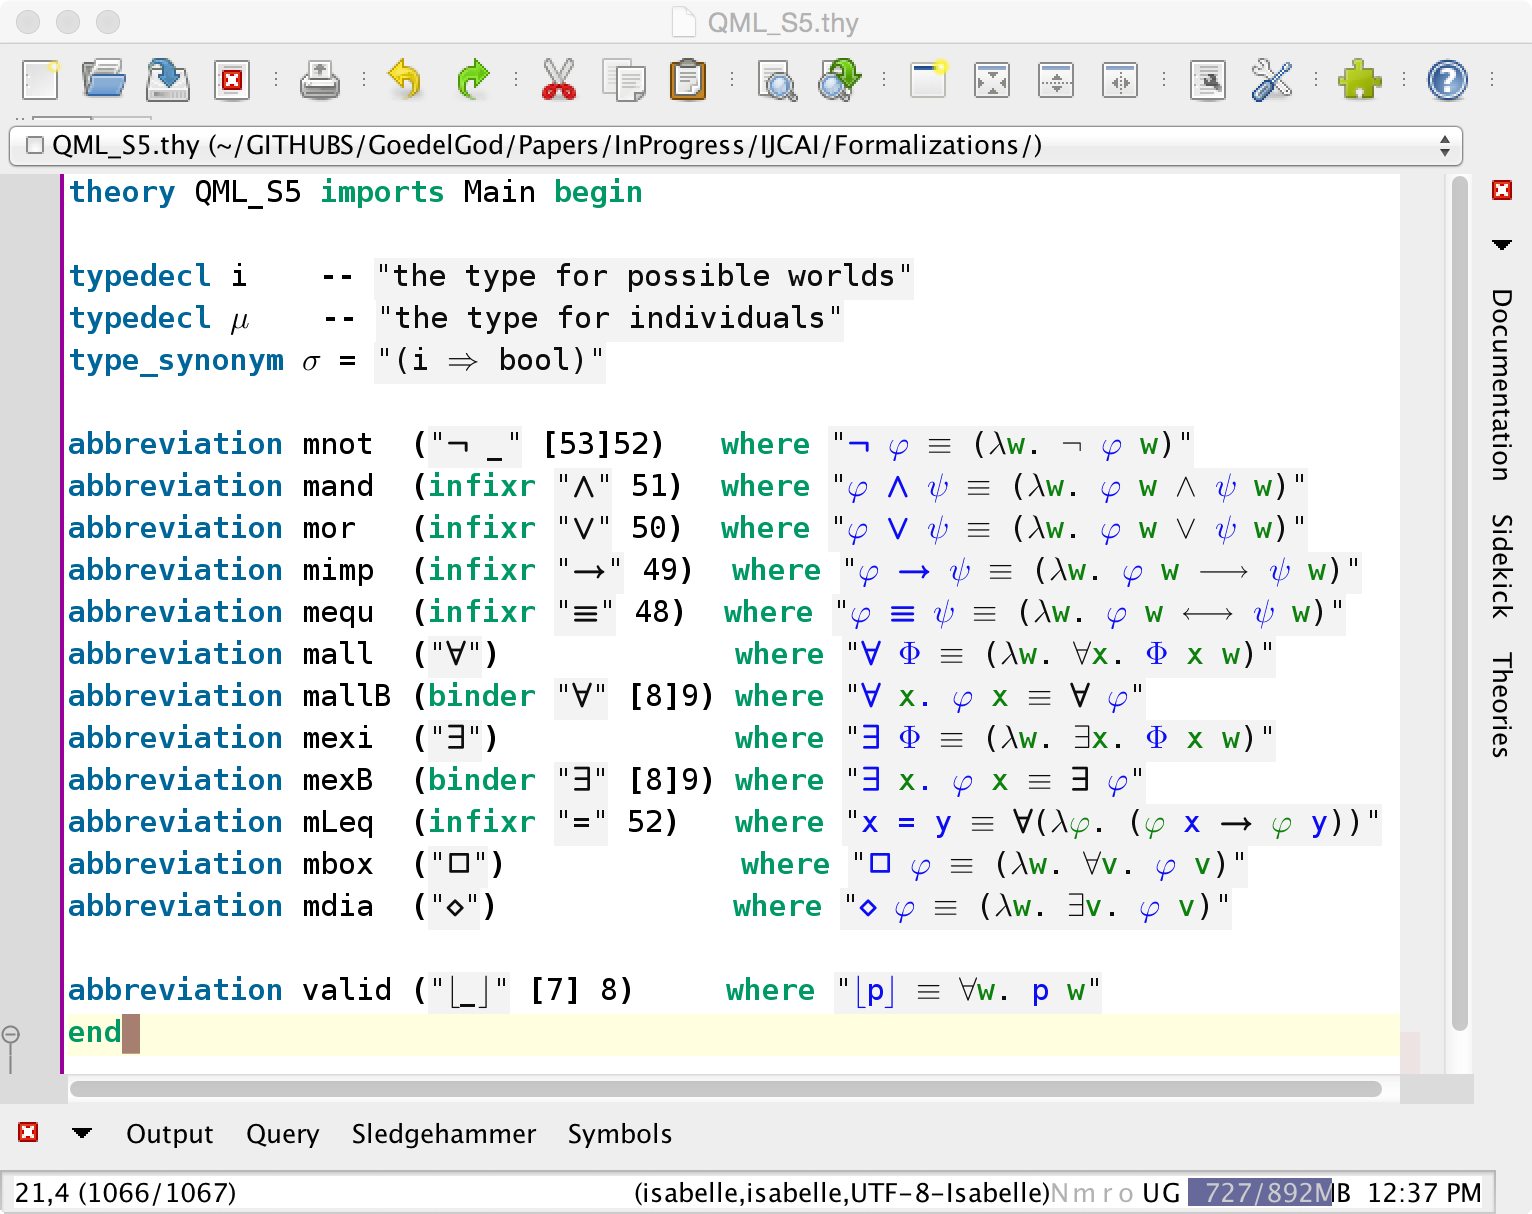
\includegraphics[width=\columnwidth]{./Images/QMLS5.png}}
\caption{Improved Embedding of S5} \label{QMLS5}
\end{figure}


\section{Full Automation of Scott's Proof}
Within the modified logic S5 Scott's proof can be fully automated. The
intermediate argumentation steps as not needed anymore to support the
prover, see Fig.~\ref{ScottS5}).
\begin{figure}
\centerline{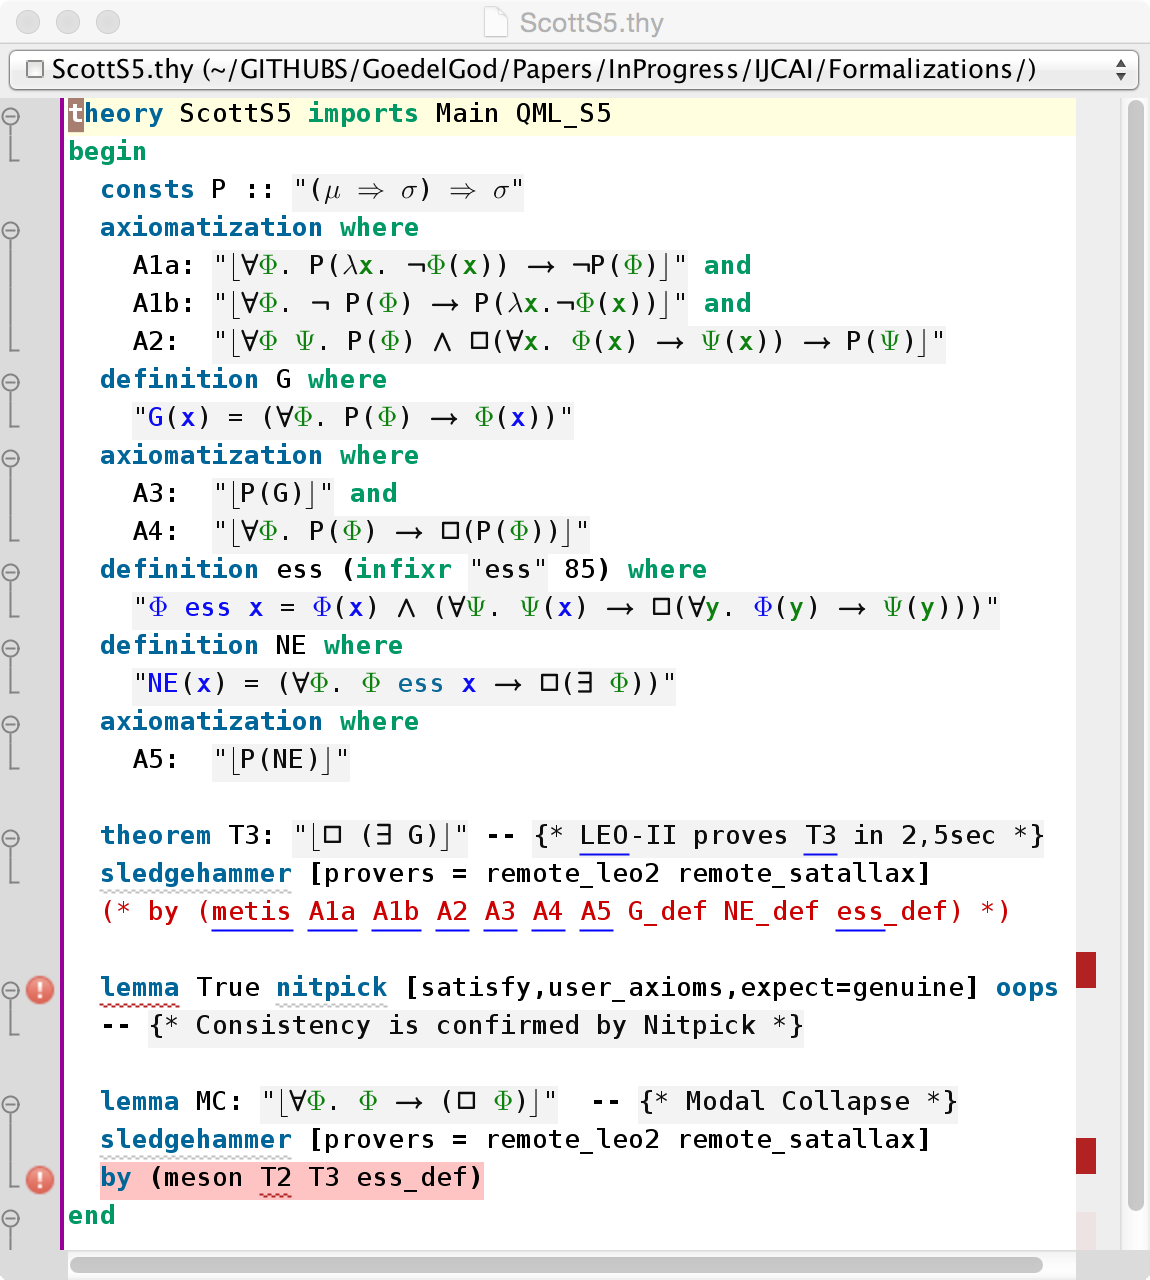
\includegraphics[width=\columnwidth]{./Images/ScottS5.png}}
\caption{Full Automation of the Ontological Argument in S5 } \label{ScottS5}
\end{figure}




In the modified S5 setting also further results can be automatically verified, which 
failed in previous work: verification of  modal collapse in
Isabelle/HOL with Meson.

\section{Intuitive Inconsistency Argument}
\subsection{LEO-II's Inaccessible Inconsistency Proof}
Tell the story (here or earlier). Show parts of LEO proof.  Inaccessible, but relevant knowledge
is contained.
\begin{figure*}
\centerline{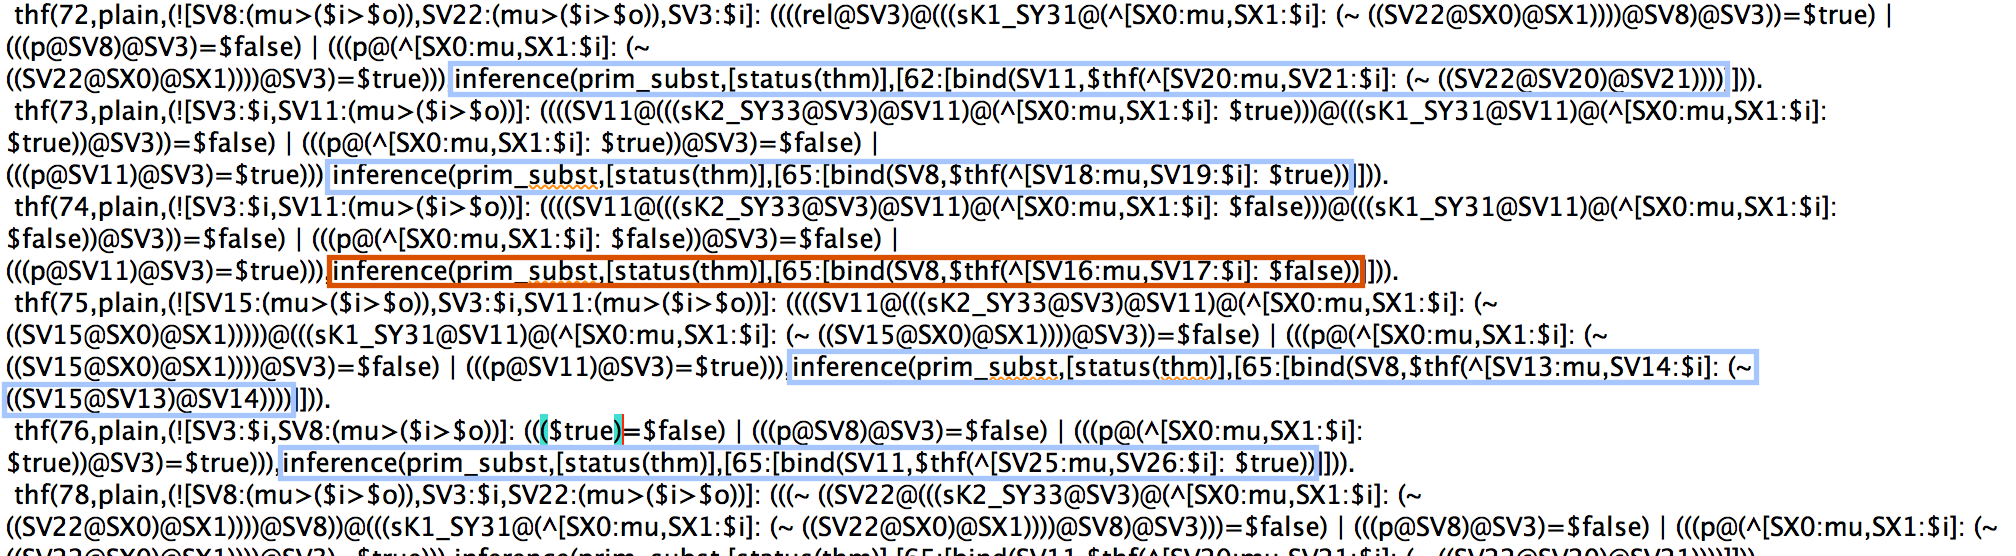
\includegraphics[width=\textwidth]{./Images/LEO-Proof.png}}
\caption{Primitive substitution in LEO-II generates candidates for the
empty property.} \label{LEO-Proof}
\end{figure*}
LEO-II's resolution proof is human unintuitive. However, it contained
relevant hints to the empty property (cf. Fig.~\ref{LEO-Proof}).

\subsection{Argument Reconstruction in Isabelle}
Present the argument informal and in Isabelle (see
Fig.~\ref{InconsistencyIsabelleK}). Easy to understand in 
in KB and KT, slightly harder in K.
\begin{figure}
\centerline{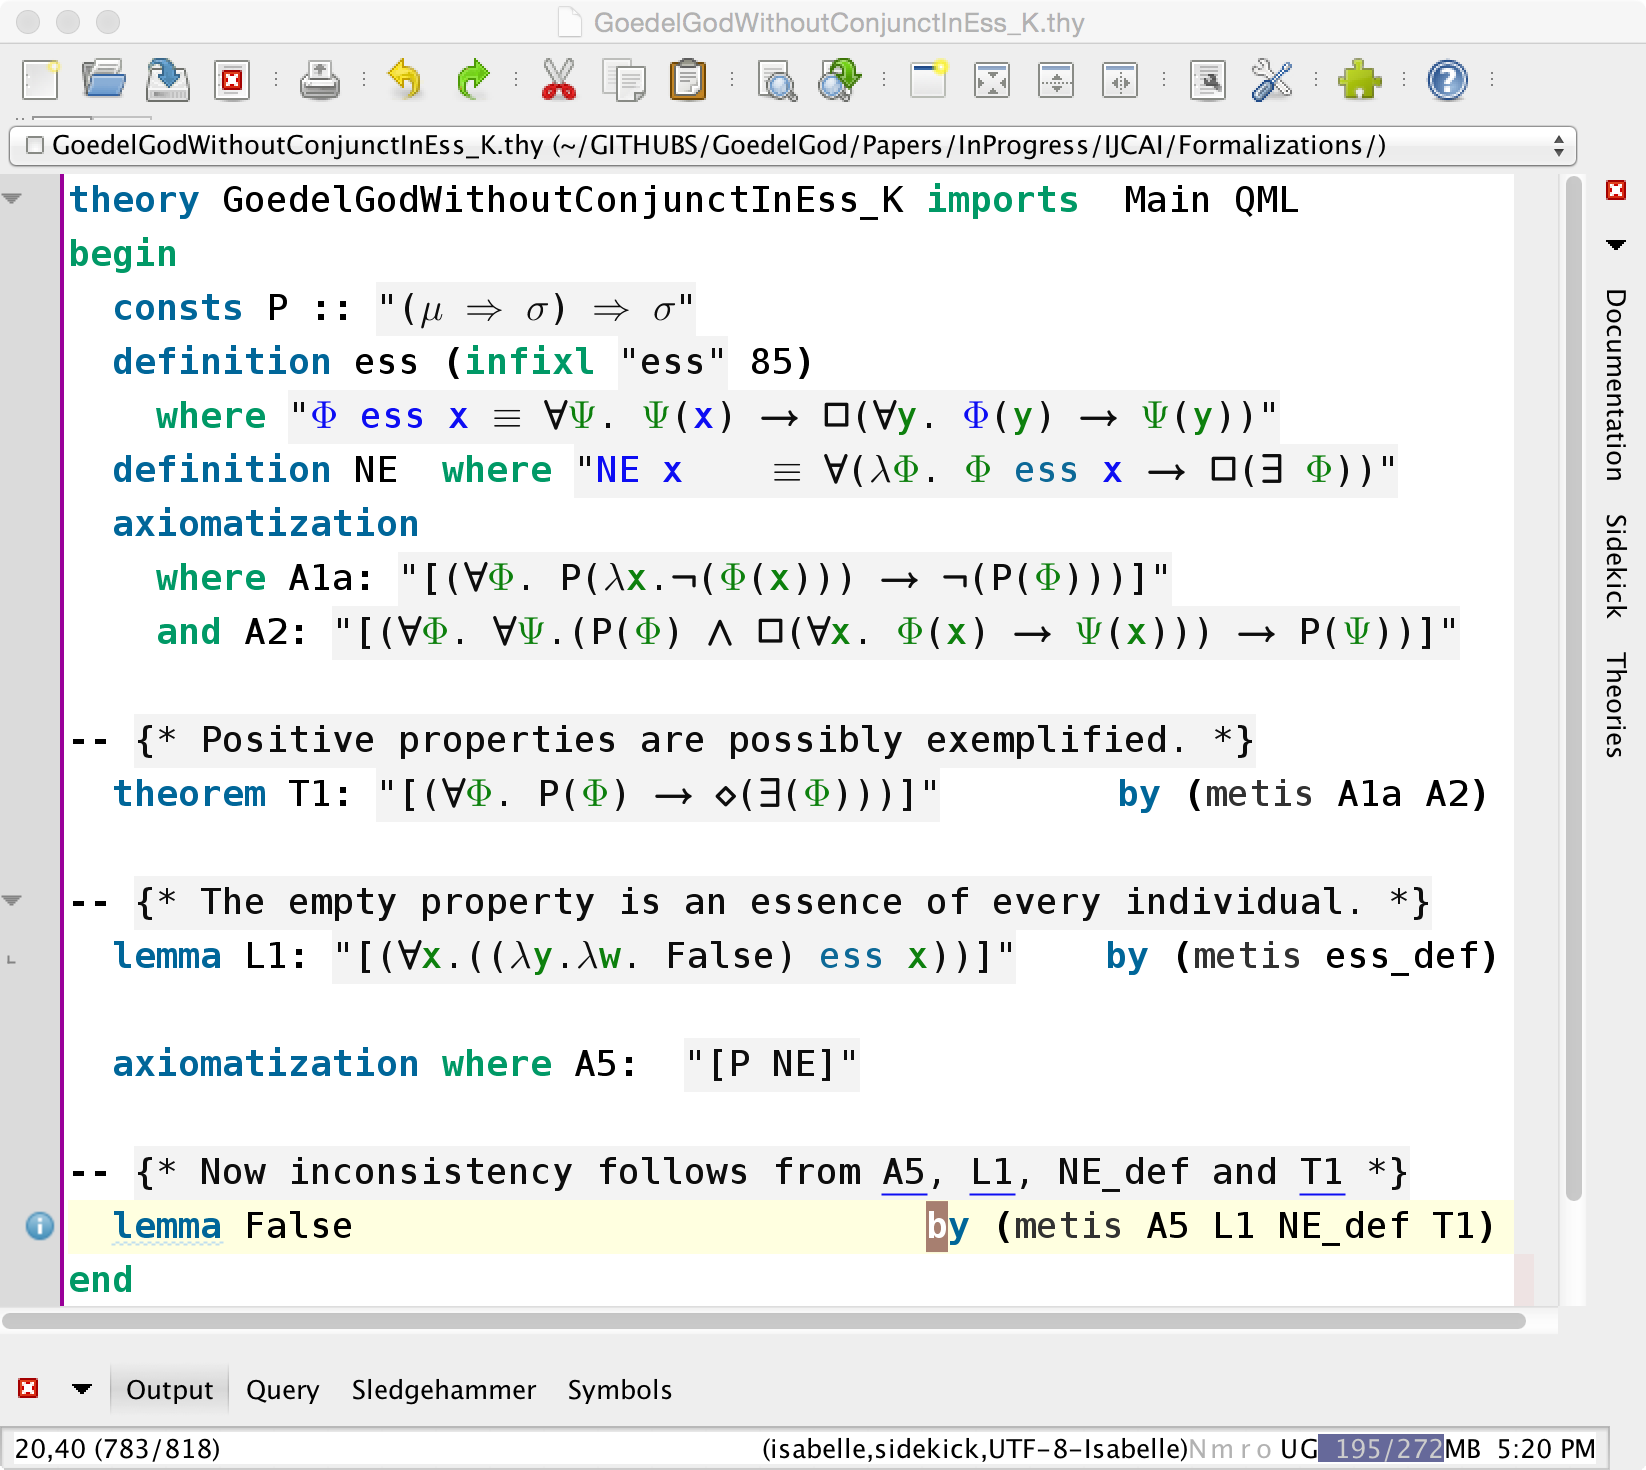
\includegraphics[width=\columnwidth]{./Images/InconsistencyIsabelleK.png}}
\caption{Reconstruction of inconsistency in Isabelle/HOl..} \label{InconsistencyIsabelleK}
\end{figure}


\subsection{Mapping to Gödel's Script}
\begin{figure*}
\centerline{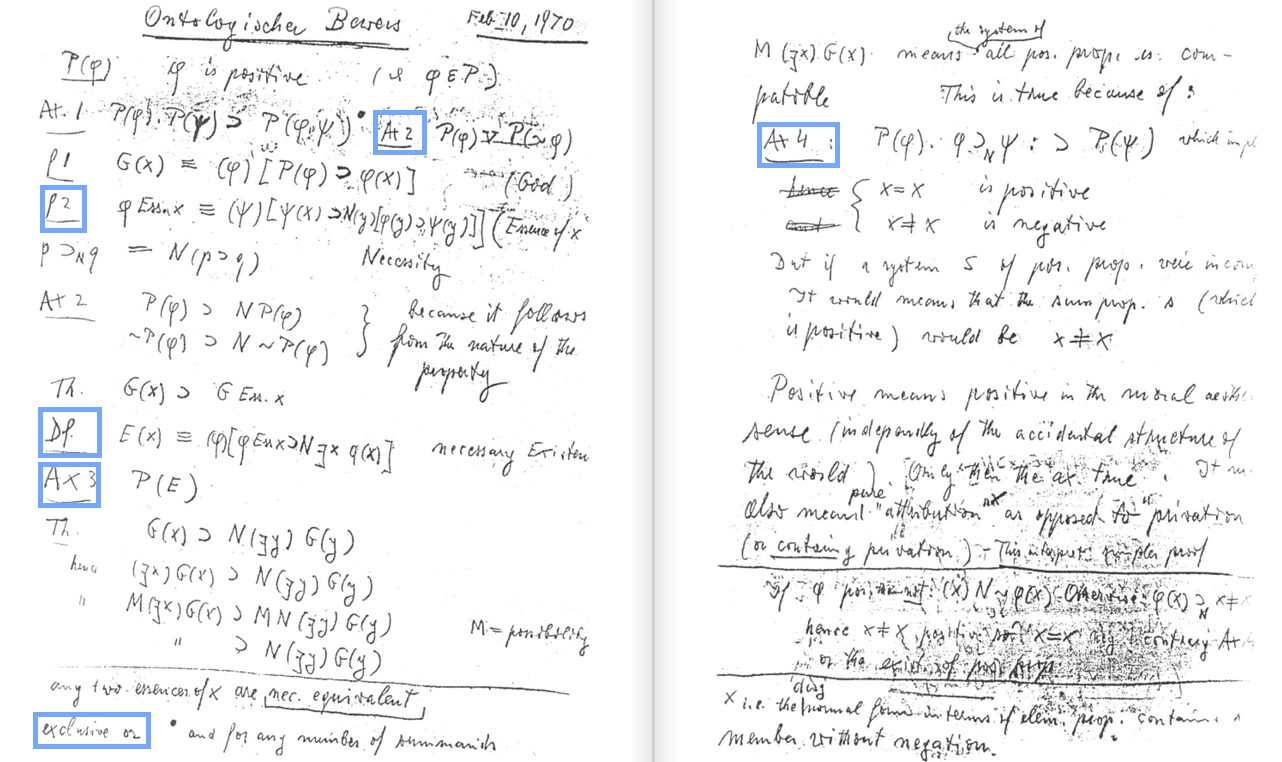
\includegraphics[width=\textwidth]{./Images/Manuscript2.png}}
\caption{Sources of Inconsistence in G\"{o}del's proof script.} \label{GoedelScript}
\end{figure*}


\section{Conclusion}


Good improvement (technical sense), Sledgehammer can still be improved
(LEO-II finds inconsistency when call directly in THF Syntax, but not
from within Isabelle). Without independent experiments directly in THF 
the inconsistency would thus not have been detected.

\section*{Acknowledgments}

Will be added at a later point.

%German Research Foundation DFG, Chad Brown

\appendix

\section{\LaTeX{} and Word Style Files}\label{stylefiles}

The \LaTeX{} and Word style files are available on the IJCAI--15
website, {\tt http://www.ijcai-15.org/}.
These style files implement the formatting instructions in this
document.

The \LaTeX{} files are {\tt ijcai15.sty} and {\tt ijcai15.tex}, and
the Bib\TeX{} files are {\tt named.bst} and {\tt ijcai15.bib}. The
\LaTeX{} style file is for version 2e of \LaTeX{}, and the Bib\TeX{}
style file is for version 0.99c of Bib\TeX{} ({\em not} version
0.98i). The {\tt ijcai15.sty} file is the same as the {\tt
ijcai07.sty} file used for IJCAI--07.

The Microsoft Word style file consists of a single file, {\tt
ijcai15.doc}. This template is the same as the one used for
IJCAI--07.

These Microsoft Word and \LaTeX{} files contain the source of the
present document and may serve as a formatting sample.  

Further information on using these styles for the preparation of
papers for IJCAI--15 can be obtained by contacting {\tt
pcchair15@ijcai.org}.

%% The file named.bst is a bibliography style file for BibTeX 0.99c
\bibliographystyle{named}
\bibliography{Bibliography}

\end{document}

